\newpage

\section{Deep Embedding Visualization}
\label{sec5}

\subsection{Theoretical motivations}

\subsubsection{From occlusion maps to visualizing embeddings}

While attributions methods (e.g. Saliency Maps, Occlusion Maps, LRP, DeepLIFT, Grad-CAM) have shown promising results for decoding individual predictions and identifying "Clever Hans" correlations thus improving the transparency of deep convolutional neural networks (DCNN), scaling such methods on large-scale datasets would unrealistically require a human operator to process tens of thousands of heatmaps as shown in \cite{Lapuschkin_2019}.

A more comprehensive visualization framework for Explainable AI would require complementing attribution methods with more holistic approaches in order to get a sense of how DCNNs internally assimilate and understand the input data its fed with. More specifically and following \cite{Rauber2017VisualizingTH}, we wish to monitor how well DCNNs perform the subsequent tasks:

\begin{itemize}
	\item \textbf{T1}: \textbf{Class Discrimination}. As we are in a multi-class classification setting, we wish to assess how well DCNNs are able to successfully disentangle labels from an originally messy input data space as shown in \cite{Rauber2017VisualizingTH} and understand prediction failure such as DCNNs on the ImageNet Dataset struggling to distinguish "missiles" from "projectiles" (as shown in Figure \ref{fig:HRV_001_Class_Hiearchy}) due to redundancies between both target labels as seen in \cite{Alsallakh2017Hierarchy}.
	
	\vspace{0.4cm}
	
	\begin{figure}[H]
		\centering
		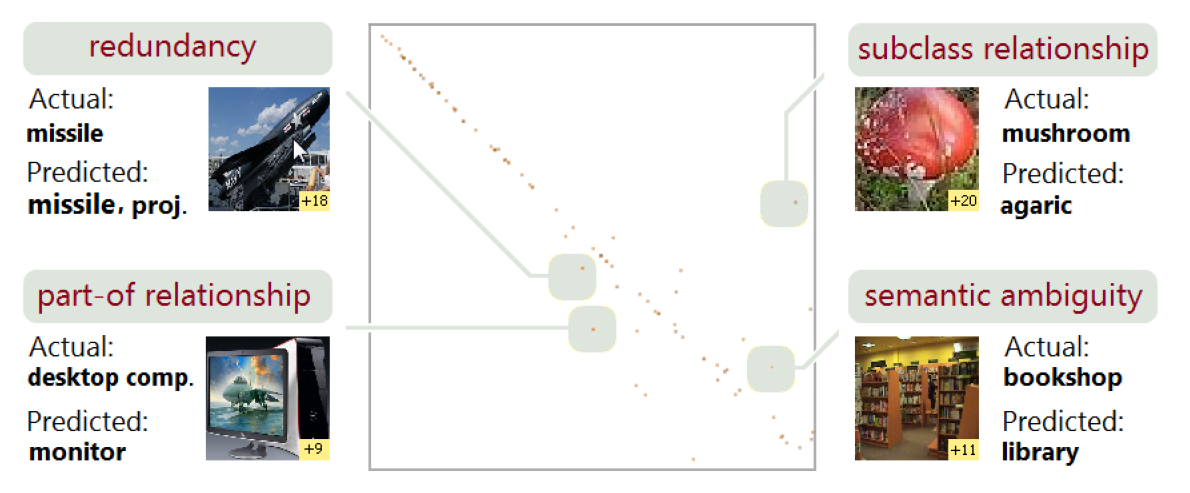
\includegraphics[scale=0.5]{images/embedding_view/HRV_Fig_001_Class_Hiearchy.PNG}
		\caption{Class confusion on ImageNet, source: \cite{Alsallakh2017Hierarchy}}
		\label{fig:HRV_001_Class_Hiearchy}
	\end{figure}
	
	\vspace{0.1cm}
	
	\item \textbf{T2}: \textbf{Neuron/Convolutional Filter Specialization}. Although state-of-the-art Deep Learning models favour overparameterization, awareness in how thousands of neurons/filters behave over differing labels as studied in \cite{Rauber2017VisualizingTH} and the existence (or not) of dead regions as highlighted by \cite{Pezzotti2018DeepEyesPV} is of keen importance for model designers.
\end{itemize}

In this regard, we found Embedding Visualization to be a suitable method for monitoring \textbf{T1} and \textbf{T2}. From \cite{Smilkov2016EmbeddingPI}, an embedding can be defined as a "map from input data to points in Euclidean space". One key strength of embeddings is that they can be used to map any given input (e.g. images, text, audio, categorical variables, graphs) into high-dimensional vectors, which can then be seamlessly projected in 2D or 3D space for user visualization with the help of dimensionality reduction methods (e.g. PCA, t-SNE, UMAP).

\subsubsection{Embeddings}

As stated by \cite{Smilkov2016EmbeddingPI}, machine learning algorithms relying on embeddings for encoding the concept of similarity between observations can be made visually accessible and easily interpretable by simply inspecting embeddings for scrutinizing and interpreting model behaviour, namely "local neighbourhoods" (how does our model perceive similar looking images?), "global geometry" (how are similarly looking image clusters interconnected with each other?) and "meaningful directions" (can we identify the latent variables driving our data?).

As an illustration, suppose a machine learning researcher develops a content-based music recommender system where music bands are encoded as high-dimensional vectors of identical shape (embeddings). A well-performing recommender system should be able to understand that Heavy Metal bands Iron Maiden and Judas Priest would have similar embeddings. It should also be able to understand in Euclidean sense how Heavy Metal bands would be much closer to Hard Rock bands than Folk or R\&B.

Widespread in Natural Language Processing for encoding word similarity (e.g. Word Embeddings and Transformers such as Word2Vec, Glove, BERT, XLNET), the concept of embeddings can also be extended to computer vision and DCNNs for encoding image similarity.

As shown on Figure \ref{fig:HRV_003_Mallat_CNN}, DCNNs are essentially functions that send their input data into a series of nonlinear convolutional operators (outputting hidden layer activations), progressively linearising the original input data to a more lower-dimensional manifold where the labels are more easily separable (through linear classifiers). This is akin to kernel methods that map nonlinear input spaces into linearly separable RKHS (albeit higher-dimensional). The difference here is that the outputs of each and every one of those intermediate convolutional operators (i.e. hidden layer activations) can be extracted as high-dimensional vectors.

\vspace{0.2cm}

\begin{figure}[H]
\centering
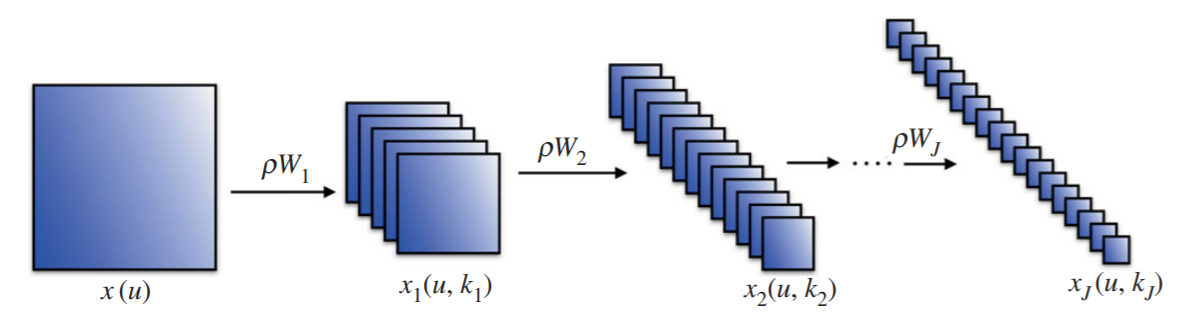
\includegraphics[scale=0.6]{images/embedding_view/HRV_Fig_003_Mallat_CNN.PNG}
\caption{A convolutional neural network: a sequence of nonlinear convolutional transformations, source: \cite{Mallat2016UnderstandingDC}}
\label{fig:HRV_003_Mallat_CNN}
\end{figure}

\vspace{0.2cm}

Thus, as pointed out by \cite{Hohman2019VisualAI}, the hidden layers of DCNNs (and by extension all Deep Learning architectures) can be viewed as embeddings (which we will then on denote as neural embeddings). This interpretation of hidden layers as embeddings has powerful implications: machine learning researchers can access those hidden layer activations as high-dimensional vectors and then visually assess them through dimensionality reduction on a 2D or 3D scatterplot. Nearly analogous to the music band recommendation example, a well-performing DCNN (as shown on Figure \ref{fig:HRV_002_Embedding_View}) should be able to perceive images from different dog breeds as having similar embeddings (i.e. images close in Euclidean space) and dog breed images as having highly dissimilar embeddings to those from ocean promontories.

\vspace{0.2cm}

\begin{figure}[H]
	\centering
	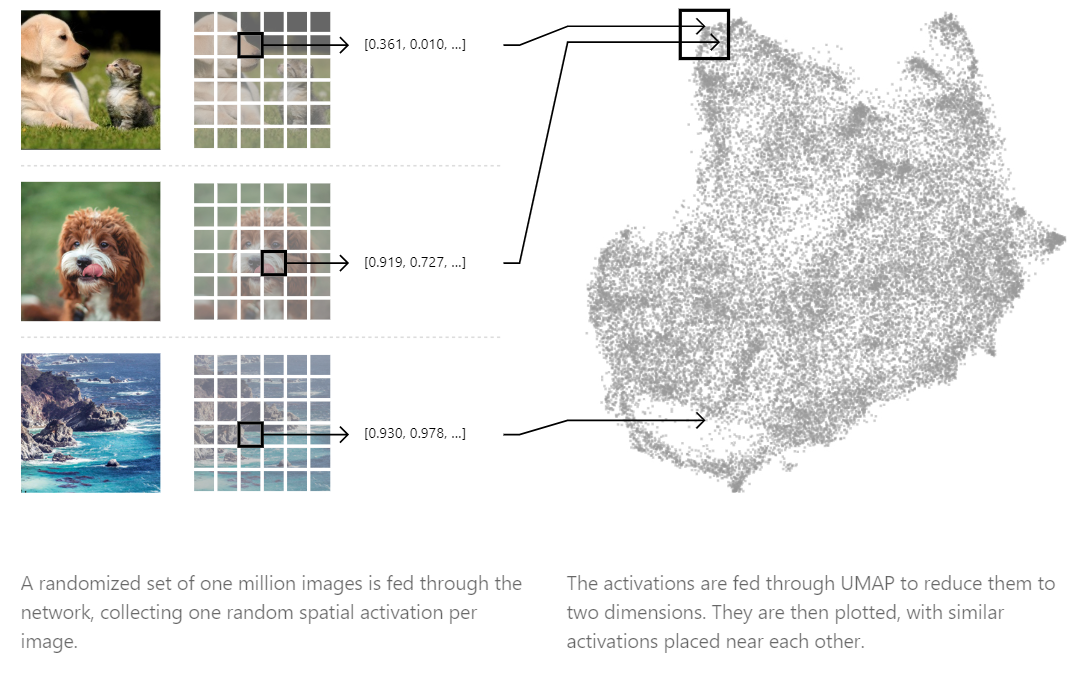
\includegraphics[scale=0.7]{images/embedding_view/HRV_Fig_002_Embedding_View.PNG}
	\caption{Randomly sampled hidden activations from InceptionV1 (mixed4c layer) projected into 2D with UMAP, source: \cite{Carter2019}}
	\label{fig:HRV_002_Embedding_View}
\end{figure}

\vspace{0.2cm}

A number of research papers across different Computer Vision fields have utilized embedding visualisation for illustrating experimental results including but not limited to:

\begin{itemize}
	\item \textbf{Deep Reinforcement Learning}: \cite{Zahavy2016GrayingTB}
	\item \textbf{Domain Adaptation}: \cite{ganin2015domainadversarial}, \cite{Sener2016LearningTR}, \cite{Li2017RevisitingBN}; \cite{Li2018ExtractingRB}
	\item \textbf{Adversarial Robustness Training}: \cite{Chen2019ImprovingAR}; \cite{Mustafa2019AdversarialDB}
	\item \textbf{Deep Metric Learning}: \cite{Song2016DeepML}; \cite{Wang2017DeepML}
\end{itemize}

A number of open-source and in-house visual analytics software also use embedding display as a major feature of their visualization framework:

\begin{itemize}
	\item \textbf{Embedding Projector (Tensorboard)}: \cite{Smilkov2016EmbeddingPI}
	\item \textbf{RevaCNN}: \cite{ChungReVACNN2016}
	\item \textbf{ActiViz (Facebook)}: \cite{Kahng2018ActiVisVE}
	\item \textbf{DeepEyes}: \cite{Pezzotti2018DeepEyesPV}
	\item \textbf{TopoAct}: \cite{Rathore2019TopoActET}
	\item \textbf{Summit}: \cite{hohman2020summit}
\end{itemize}

Embedding visualization sits nicely with recent work on biological interpretations of how DCNNs operate and the need for deeper architectures. As detailed in \cite{Mallat2016UnderstandingDC}, DCNNs subjects its input image data to a series of linear operations through convolutional filters followed by nonlinear transformations through activation functions. Such operations help further linearise an initially high-dimensional input space ($\mathbb{R}^{3072}$ on CIFAR-10 and $\mathbb{R}^{196608}$ on ImageNet) such that at the end of our sequence, the newly linearised input data can easily be separated with a linear classifier (e.g. logistic/softmax classifier). This linearisation capacity has seen interesting analogies with the primate visual cortex's ability of progressively flattening high-dimensional object manifolds such that the brain can easily discriminate between objects, as seen in \cite{DiCarlo2007UntanglingIO} and \cite{Cohen2020SeparabilityAG}. The brain's faculty of easily discerning objects from originally intricate images has even been represented as a linear hyperplane separator as seen in Figure \ref{fig:HRV_004_Cortex_View}.

\vspace{0.2cm}

\begin{figure}[H]
	\centering
	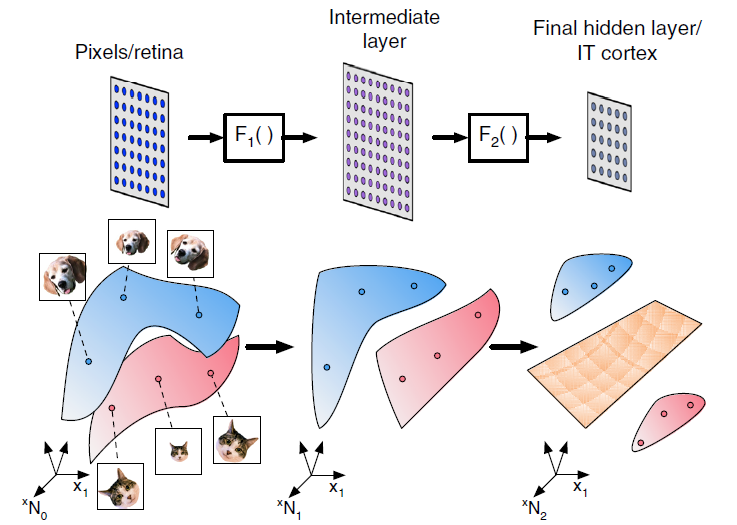
\includegraphics[scale=0.8]{images/embedding_view/HRV_Fig_004_Visual_Cortex.PNG}
	\caption{Linearisation of high-dimensional object manifolds (labelled input images) with DCNNs, source: \cite{Cohen2020SeparabilityAG}}
	\label{fig:HRV_004_Cortex_View}
\end{figure}

\vspace{0.2cm}

This gives us a useful heuristic for monitoring the convolutional layers' internal behaviour: the more visually separated the embeddings in 2D space are, the likelier we can posit that our DCNN is capable of discriminating the classes it was programmed to distinguish.

\subsubsection{Embedding Visualization: Dense Layers}

There were early attempts from \cite{Hinton2006}, \cite{Maaten2014AcceleratingTU} and \cite{aubry2015understanding} to project neural embeddings from Dense (or Fully-Connected) Layers into 2D space with dimensionality reduction algorithms (PCA, t-SNE) for inspecting neural network behaviour. Notwithstanding, many research papers and visual analytics frameworks that rely on visualizing dense layer embeddings often cite work from \cite{Rauber2017VisualizingTH}.

From a series of experiments on MNIST, SVHN (Street View House Numbers) and CIFAR-10 using Barnes-Hut t-SNE, \cite{Rauber2017VisualizingTH} helped frame some of the key benefits of visualizing dense layer embeddings: first, dense embedding visualisation provides intuitive visual feedback essentially since for the image embeddings we are projecting into 2D space we have access to their labels, thus we can easily assess whether the embeddings learned by our neural networks are able to successfully discriminate labels. This is useful for monitoring the training phase of DCNNs as seen on Figure \ref{fig:HRV_006_Rauber_B}: as the training phase progresses, the embeddings learned by our DCNN become increasingly class-relevant. We can visually infer this on our embedding scatter plot as the class digit clusters becoming increasingly distant from each other. Overlapping clusters would indicate that our model is confusing two classes with one another.

\vspace{0.2cm}

\begin{figure}[H]
	\centering
	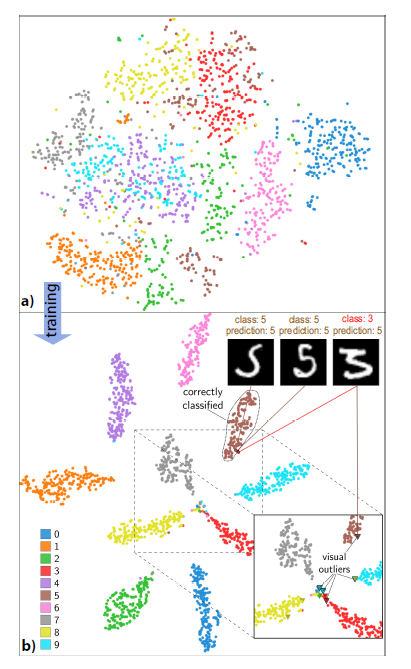
\includegraphics[scale=0.9]{images/embedding_view/HRV_Fig_006_Rauber_B.PNG}
	\caption{Barnes-Hut t-SNE Projection of LeNet5 Before and After Training on Digits MNIST, source: \cite{Rauber2017VisualizingTH}}
	\label{fig:HRV_006_Rauber_B}
\end{figure}

\vspace{0.2cm}

Dense embedding visualisation can also be used to explain model failure, which can provide visual feedback as shown on Figure \ref{fig:HRV_005_Rauber_A}:

\vspace{0.2cm}

\begin{figure}[H]
	\centering
	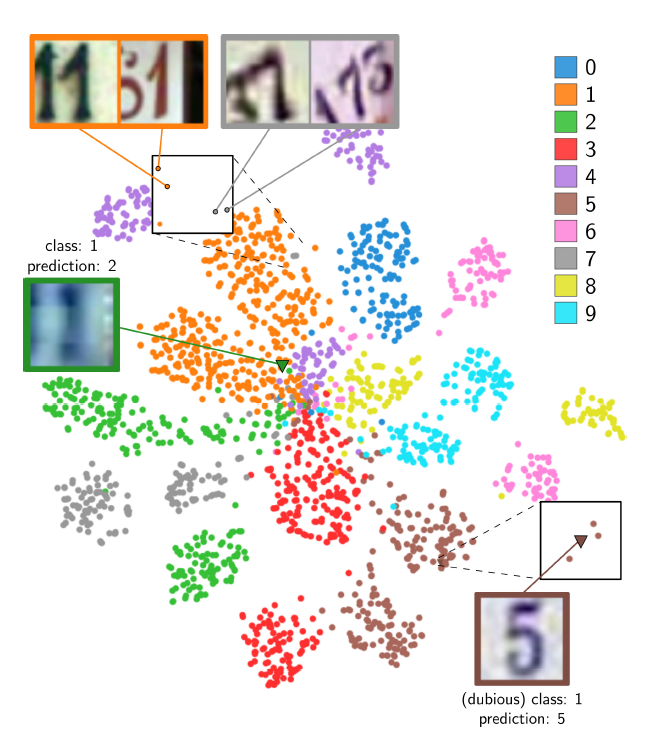
\includegraphics[scale=0.65]{images/embedding_view/HRV_Fig_005_Rauber_A.PNG}
	\caption{Barnes-Hut t-SNE Projection of LeNet5 Before and After Training on SVHN, source: \cite{Rauber2017VisualizingTH}}
	\label{fig:HRV_005_Rauber_A}
\end{figure}

\vspace{0.2cm}

Error analysis on Figure \ref{fig:HRV_005_Rauber_A} can help identify anomalies in our training process and even dataset quality: confusing inputs with different labels cluttering all over the image, similarly looking classes that nevertheless were labelled differently or labelling mistakes (e.g. a clear Digit 5 incorrectly labelled in the validation set as a Digit 1), etc.

The authors do point out a number of caveats to watch out: first, Barnes-Hut t-SNE needed 10 minutes to compute the 2D projections, which while fair for static analysis would be to slow and impractical for a Tensorboard-style framework designed to monitor the training phase of DCNNs. Issues with scalability also pop up when the number of classes are very high (e.g. CIFAR-100, ImageNet). The categorical colour mapping - for assessing how well our model is able to discriminate between different labels - will quickly create visual clutter on our scatter plot, which a continuous colour mapping is unlikely to fix. Finally, while the authors found that embedding visualisation usually led to insightful visual feedback on internal model behaviour, there are no guarantees of success for unsupervised learning methods such as dimensionality reduction and without supplementary metrics from supervised learning (such as accuracy scores for each class, confusion matrices), such visualisations could be misleading.

\subsubsection{Embedding Visualization: Convolutional Layers}
\label{embeddings-convolutional}

Convolutional layer embeddings present a much harder challenge. Dense layer activations can be extracted as matrices, but convolutional layers output multi-channel hidden activations which can be extracted not as matrices but 3D tensors. The most readily-used dimensionality reduction algorithms can only reduce the dimensionality of matrices, not tensors. This explains why until recently the focus of embedding visualisation was exclusively on dense embeddings, as they are easier to plot.

In recent years, there have been attempts to extract the hidden activations of convolutional layers and reduce them to a lower-dimensional space for visualisation. \cite{Pezzotti2018DeepEyesPV} developed DeepEyes' for monitoring the training phase of DCNNs following guidelines from Progressive Visual Analytics. They expanded on initial work over embedding visualisation from \cite{Rauber2017VisualizingTH} for convolutional layers. They randomly sample tens of thousands of patches for each image (known as receptive fields), obtain activations for said patches and project those activations into lower-dimensional space for visualisation with a faster C++ implementation of t-SNE (called Hierarchical t-SNE). As seen on Figure \ref{fig:HRV_007_Pezzotti_A}, we find a similar conclusion to Figure \ref{fig:HRV_006_Rauber_B}: deeper layers tend to be more class specialized, whereas parameter/filter sharing is more prevalent in earlier layers.

\vspace{0.2cm}

\begin{figure}[H]
	\centering
	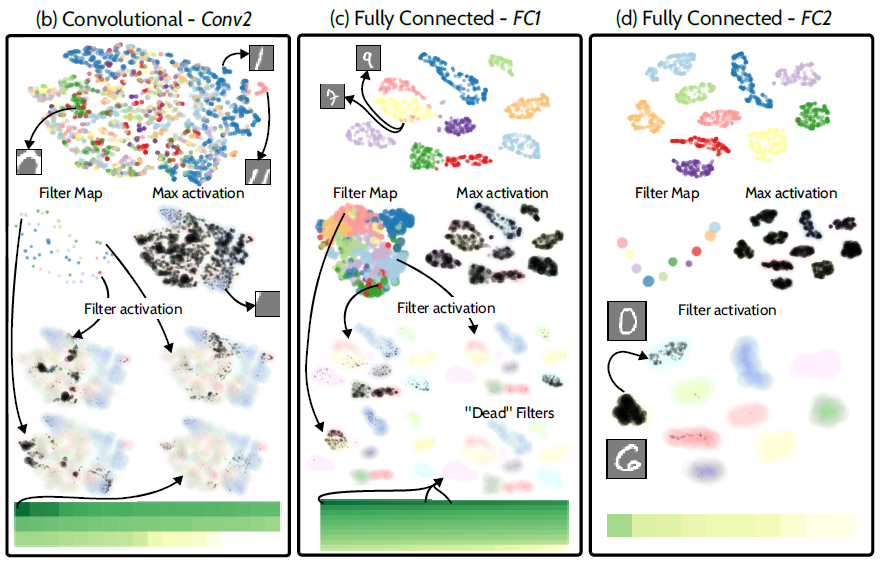
\includegraphics[scale=0.75]{images/embedding_view/HRV_Fig_007_Pezzotti_A.PNG}
	\caption{Hierarchical t-SNE Projection of LeNet5 Layers Before and After Training on MNIST, source: \cite{Pezzotti2018DeepEyesPV}}
	\label{fig:HRV_007_Pezzotti_A}
\end{figure}

\vspace{0.2cm}

This approach for extracting the hidden activations was also utilized by \cite{Carter2019} and \cite{Rathore2019TopoActET} for decoding InceptionV1 on ImageNet. Instead of projecting the receptive fields and plotting them with their respective labels, they run their own feature visualisation techniques on top of those receptive fields. This allows them to explicitly highlight how DCNNs start by detecting edges and textures before moving in later layers to full objects.

Contrasting the aforementioned approaches, \cite{hohman2020summit} - for their visual analytics software Summit - take a different approach: the authors focus on extracting the most useful information out of the convolutional layers channel depth. The authors start by assuming that channels can be more or less interpreted as concepts (e.g. edges, textures, patterns, parts of objects) and that for a given image fed through the convolution layer, the higher the activation values the more representative the concept within the image. As an illustration, for a batch of images passed through a 512-channel convolutional layer, only the maximal activation value is kept for each of the 512 channels. The authors hold that this operation is equivalent to running a Global Maximum Pooling over each layer.

Therefore, images fed through a 512-channel convolutional layer can be described as a 512-dimensional channel vector. This solves the roadblock of representing tensor-shaped convolutional layer activations as high-dimensional vectors. The authors go even further and aggregate each channel vector per class, creating a class-activation matrix, which they then plot down into 2D with UMAP as seen on Figure \ref{fig:HRV_008_Summit}.

\vspace{0.2cm}

\begin{figure}[H]
	\centering
	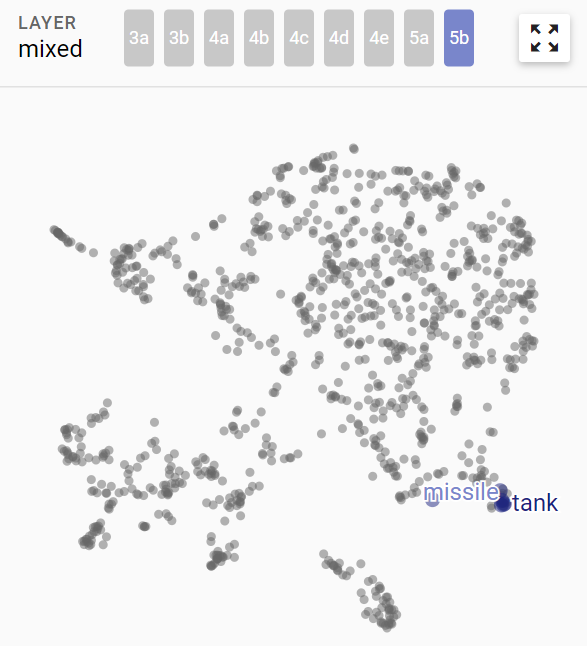
\includegraphics[scale=0.85]{images/embedding_view/HRV_Fig_008_hohman_UMAP.PNG}
	\caption{UMAP Projection of InceptionV1 Mixed5b Layer on ImageNet, source: \cite{hohman2020summit}}
	\label{fig:HRV_008_Summit}
\end{figure}

\vspace{0.2cm}

One major benefit of this approach is that it scales well with an extremely high number of classes as seen on Figure \ref{fig:HRV_008_Summit} with ImageNet dataset's 1000 classes.

\subsubsection{Embedding Visualization: Neuron/Filter Activity}

One limitation of the aforementioned visualizations (at a layer level) is that it ignores examining the relationships between the different filters or neurons and how those groups of parameters interact between each other in order to accomplish their roles (e.g. classification, regression, generative modelling). In light of this, \cite{Rauber2017VisualizingTH} offered a novel approach (at least at the time and for dense layers only) to visualizing how similar neurons co-interact with each other and how dissimilar neurons are in Euclidean sense far apart.

Using the same extraction procedure for visualizing the hidden representations learned by the DCNN, they treat each neuron as a vector described by $n$ layer activations, they start by computing a Pearson correlation matrix $\rho$ between neuron pairs. From this correlation matrix, they compute dissimilarity scores $1 - |\rho_{i,j}|$ for each neuron pair $i$ and $j$. From this dissimilarity matrix of neurons, they project this matrix down to 2D with the help of multidimensional scaling (MDS). MDS is more suited for preserving global relationships between our original data when reduced to a lower-dimensional space. And as the number of dimensions to reduce are small (less than a thousand neurons), the procedure is not bottlenecked by its quadratic complexity of $O(n^2)$. They obtain the following visualization (as seen in Figure \ref{fig:HRV_009_Neuron_Spec}):

\vspace{0.2cm}

\begin{figure}[H]
	\centering
	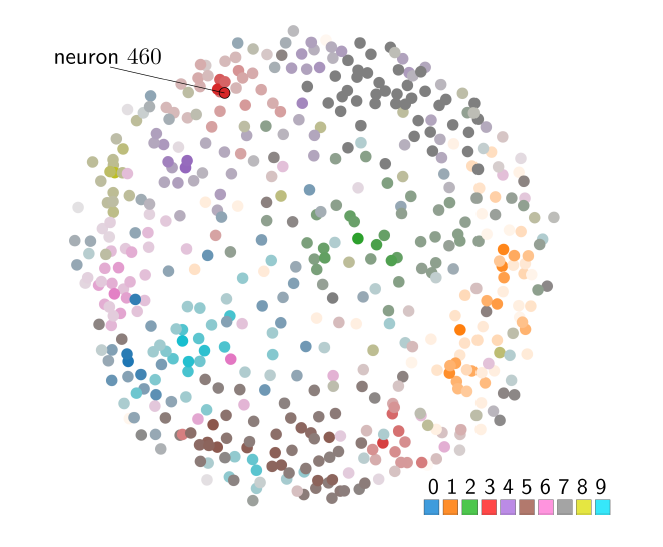
\includegraphics[scale=0.85]{images/embedding_view/HRV_Fig_009_Neuron_Spec.PNG}
	\caption{MDS Projection of Peniultimate Dense Layer Neurons, source: \cite{Rauber2017VisualizingTH}}
	\label{fig:HRV_009_Neuron_Spec}
\end{figure}

\vspace{0.2cm}

The authors highlight one potential application of such visualization: monitor how different regions of a given layer specialize for accomplishing different supervised learning tasks, e.g. on the SVHN dataset, how one set of neurons is mostly active when predicting Digit 3 whereas another region is specialized in detecting Digit 1. They accomplish this by using supervised learning (here extra-randomized trees) to output a discriminative score for each neuron, measuring the associative strength of a neuron with a given label.

The aforementioned visualization from \cite{Rauber2017VisualizingTH} only works on dense layers. \cite{Pezzotti2018DeepEyesPV} extended the aforesaid authors' work for convolutional layers.


\vspace{0.2cm}

\begin{figure}[H]
	\centering
	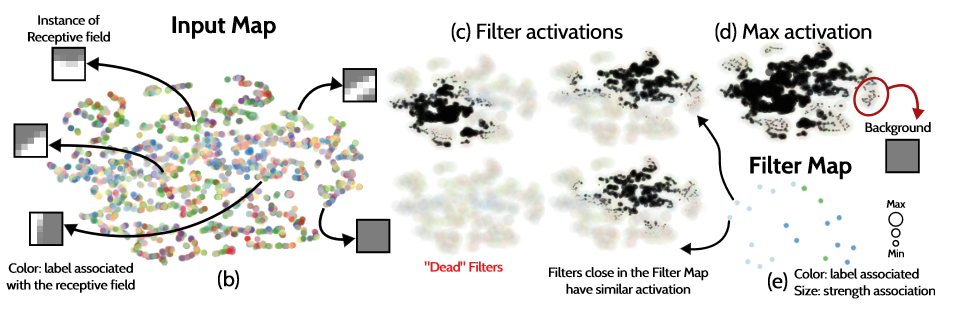
\includegraphics[scale=0.85]{images/embedding_view/HRV_Fig_010_Dead_Zones.PNG}
	\caption{Hierarchical t-SNE Projection of Convolutional Layer Activations (Input Map) and Filters (Filter Map), source: \cite{Pezzotti2018DeepEyesPV}}
	\label{fig:HRV_010_Dead_Zones}
\end{figure}


\vspace{0.2cm}

Filters structure convolutional layers, which differ significantly from dense layer neurons in that they are 3-dimensional tensors (for width, height and number of channels). Thus, \cite{Pezzotti2018DeepEyesPV} uses an alternative distance metric (different from Pearson correlation) for computing the filter similarity: a custom Jaccard similarity distance $\phi_{i,j}$ between two convolutional layer filters $i$ and $j$. Once a similarity matrix $\phi$ is computed, just as in the case of dense layers, the similarity matrix is brought down to a 2-dimensional plane (here with the help of t-SNE) and easily visualized on a 2D scatterplot. Finally, each filter is colored differently, depending on how often a filter responds to a particular label (hinting at specialization). For each filter, an internal metric (described in greater detail in the authors' paper) keeps tabs of how strongly it reacts to all labels.


An example from \cite{Pezzotti2018DeepEyesPV} is provided on Figure \ref{fig:HRV_010_Dead_Zones} through the authors' Filter Map. Interacting with a specific filter on the Filter Map highlights the observations that reacted the most strongly with the selected unit. This functionality allows model designers to quickly identify redundant filters that almost never fire off (although manually pruning superfluous units is no guarantee of improved performance).


\subsection{Interactive Viewer with Plotly Dash}

\subsubsection{Deep Embedding Viewer (i): Motivation}

To synthesize work across different research papers, an interactive prototype was developped as a synthesis and a Proof-Of-Concept of how Embedding Visualization can be put to use for different use-cases: e.g. model comparison, training phase monitoring, adversarial training, etc. An illustration of our viewer's goal is provided below (Figure \ref{fig:HRV_011_DEV_Schema}):


\vspace{0.2cm}

\begin{figure}[H]
	\centering
	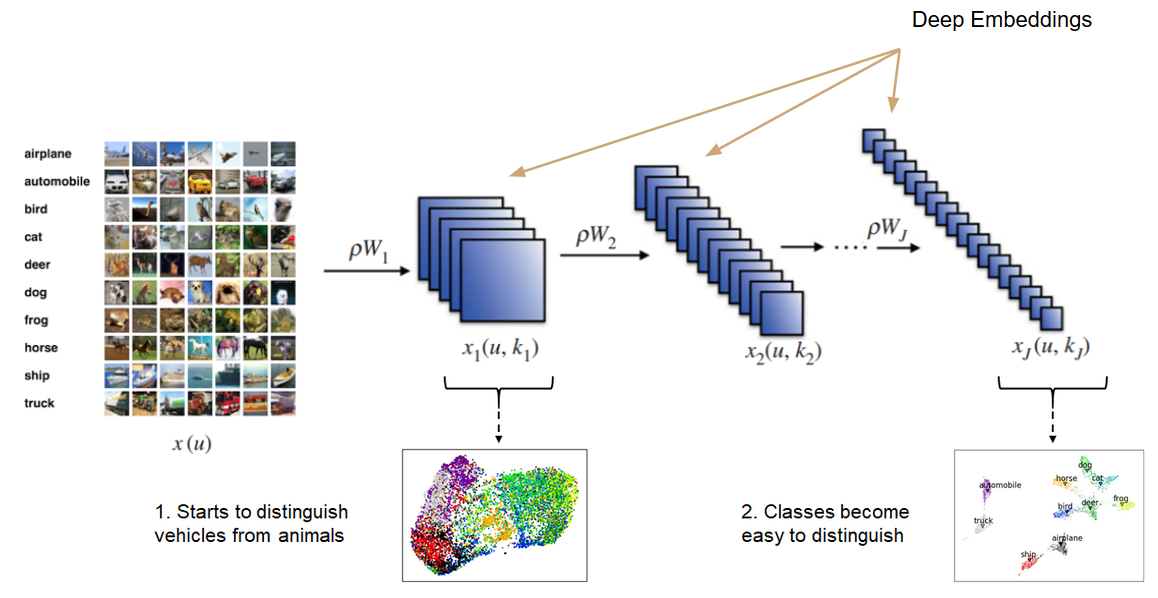
\includegraphics[scale=0.65]{images/embedding_view/HRV_Fig_011_Schema.PNG}
	\caption{Deep Embedding Viewer (with Plotly Dash): Illustrative Schema}
	\label{fig:HRV_011_DEV_Schema}
\end{figure}

\vspace{0.2cm}


Since production deployment in a real-life environment is not the purpose of this research venture, Plotly Dash was chosen as our interactive visualization library. Dash allows for quickly prototyping dashboards without the verbose development infrastructure of more sophisticated visualization frameworks (such as D3.js). 

Our interactive viewer - named \textbf{Deep Embedding Viewer} - takes a Keras model and an available dataset (limited to CIFAR-10 for this research project). Extending our viewer to Tensorflow 2.0 and PyTorch models or alternative datasets is out-of-scope. Keras models are to be dropped into a specific folder from which dropdown selection allows the user to easily select and even later swap between different models (as seen on Figure \ref{fig:HRV_011_DEV_Intro}).


\vspace{0.2cm}

\begin{figure}[H]
	\centering
	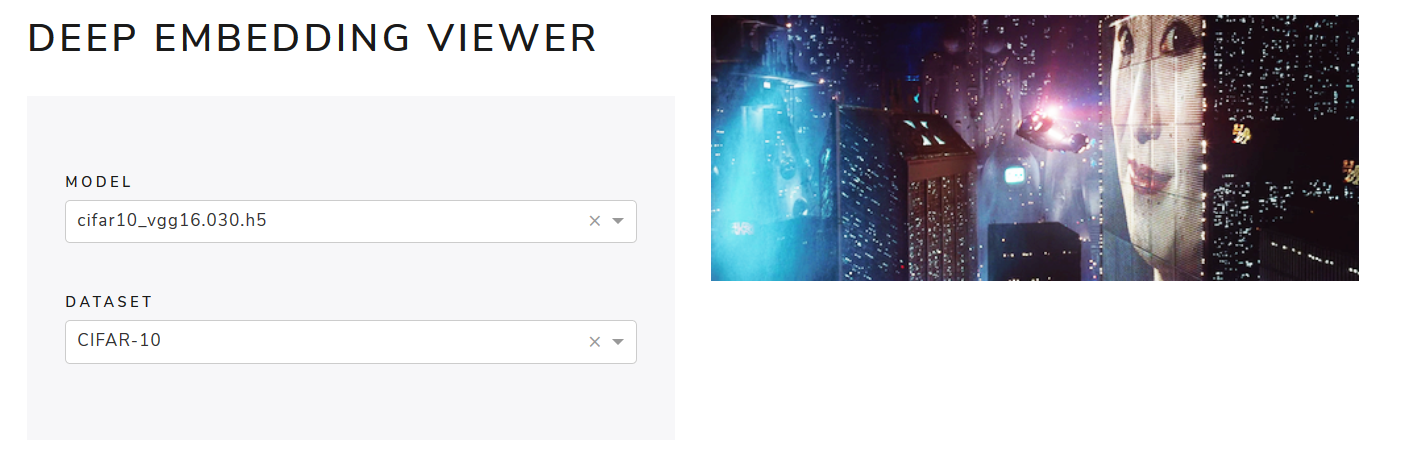
\includegraphics[scale=0.55]{images/embedding_view/HRV_Fig_011_DEV_Intro.PNG}
	\caption{Deep Embedding Viewer (with Plotly Dash): Keras Model and Dataset Selection}
	\label{fig:HRV_011_DEV_Intro}
\end{figure}

\vspace{0.2cm}

Once a model and dataset were chosen, our viewer loads a total of five panels:

\begin{enumerate}
	\item Learned Representations View
	\item Image Viewer
	\item Neuron Activity Map
	\item Model Performance Analysis
	\item Adversarial Robustness Simulation
\end{enumerate}

The viewer fully utilizes Plotly Dash's callback system for creating dependencies between the different panels, allowing for a user to swap between different models of his choosing (as seen Figure \ref{fig:HRV_Fig_019_DEV_Callback_Structure}).

\newpage


\begin{figure}[H]
	\centering
	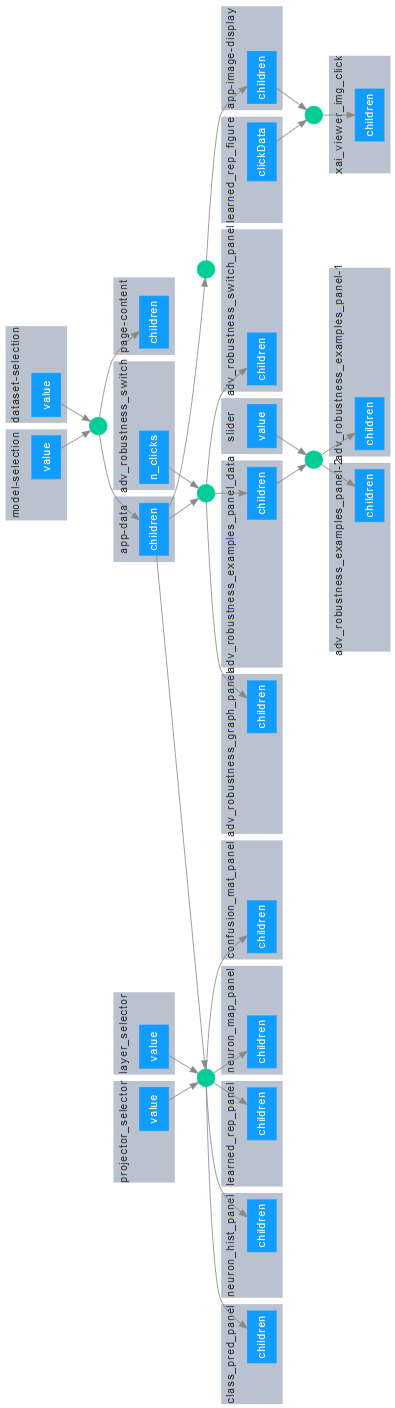
\includegraphics[scale=0.9]{images/embedding_view/HRV_Fig_019_DEV_Callback_Structure.PNG}
	\vspace{0.2cm}
	\caption{Deep Embedding Viewer (with Plotly Dash): Callback Structure}
	\label{fig:HRV_Fig_019_DEV_Callback_Structure}
\end{figure}

\newpage


\subsubsection{Deep Embedding Viewer (ii): Learned Representations View / Image Viewer}

The showcase of our viewer is the \textbf{Learned Representations View} for visualizing DCNN embeddings on a 2-dimensional scatterplot. It is heavily inspired from much of the research literature presented in the earlier subsections. It is capable of handling both dense and convolutional layers. Specifically, for dense layers, it follows closely work from \cite{Rauber2017VisualizingTH} with the sole exception that UMAP - a more computationally-efficient nonlinear dimensionality reduction algorithm - replaces t-SNE. In the case of convolutional layers, we opted for a streamlined version of the methodology implemented on \cite{hohman2020summit}, instead of the receptive field approach used instead by \cite{Pezzotti2018DeepEyesPV} and \cite{Carter2019}. The former was simply easier to implement than the latter.

Since we are interested in how our DCNN is reacting to data and understand the nature of its decision-making process, we will use a randomly sampled version of CIFAR-10 dataset's training data (forming a validation set) that was not used during the entirety of the training process.

For the scatterplot itself, Plotly Dash provides user interactivity and one such application is image display through the \textbf{Image Viewer}. In addition to colouring each embedded image with its respective label, to help reminder the viewer that the dots on the scatterplot are supposed to represent images, simply clicking on any unit will display its corresponding image. Selecting an embedding image with a correct prediction ensues the following display (Figure \ref{fig:HRV_016_DEV_Image_Viewer_1}):

\vspace{0.2cm}

\begin{figure}[H]
	\centering
	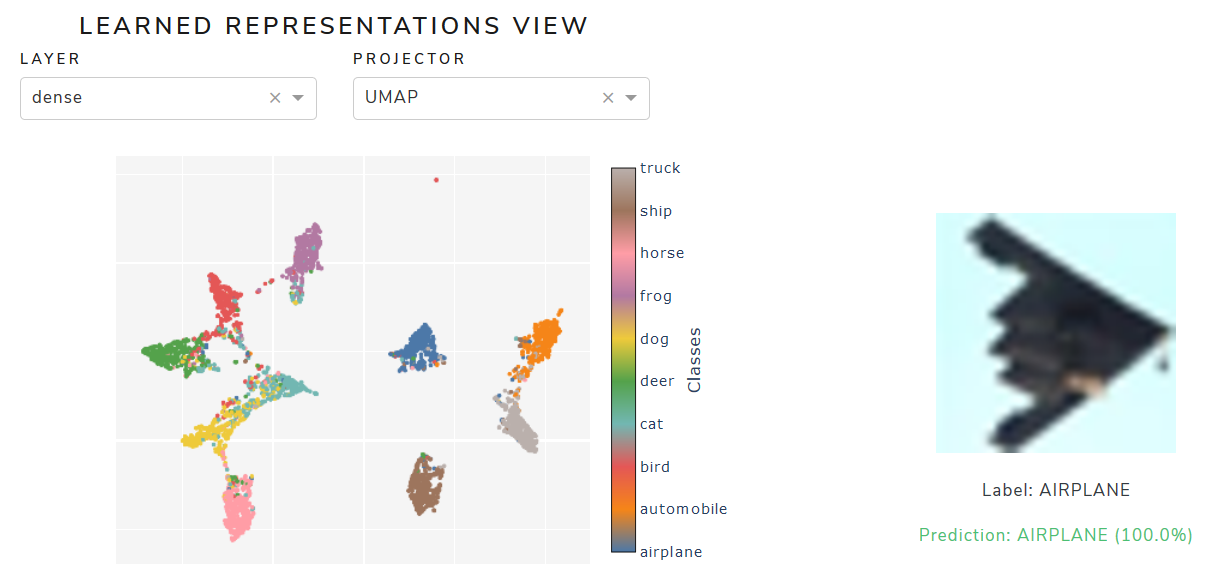
\includegraphics[scale=0.65]{images/embedding_view/HRV_Fig_016_DEV_Layer_Embedding.PNG}
	\caption{Deep Embedding Viewer (with Plotly Dash): Learned Representations View with an Accurate Prediction}
	\label{fig:HRV_016_DEV_Image_Viewer_1}
\end{figure}

\vspace{0.2cm}

Conversely, a selected embedding image with an incorrect prediction will result in the following (cf. Figure \ref{fig:HRV_016_DEV_Image_Viewer_2}):

\vspace{0.2cm}

\begin{figure}[H]
	\centering
	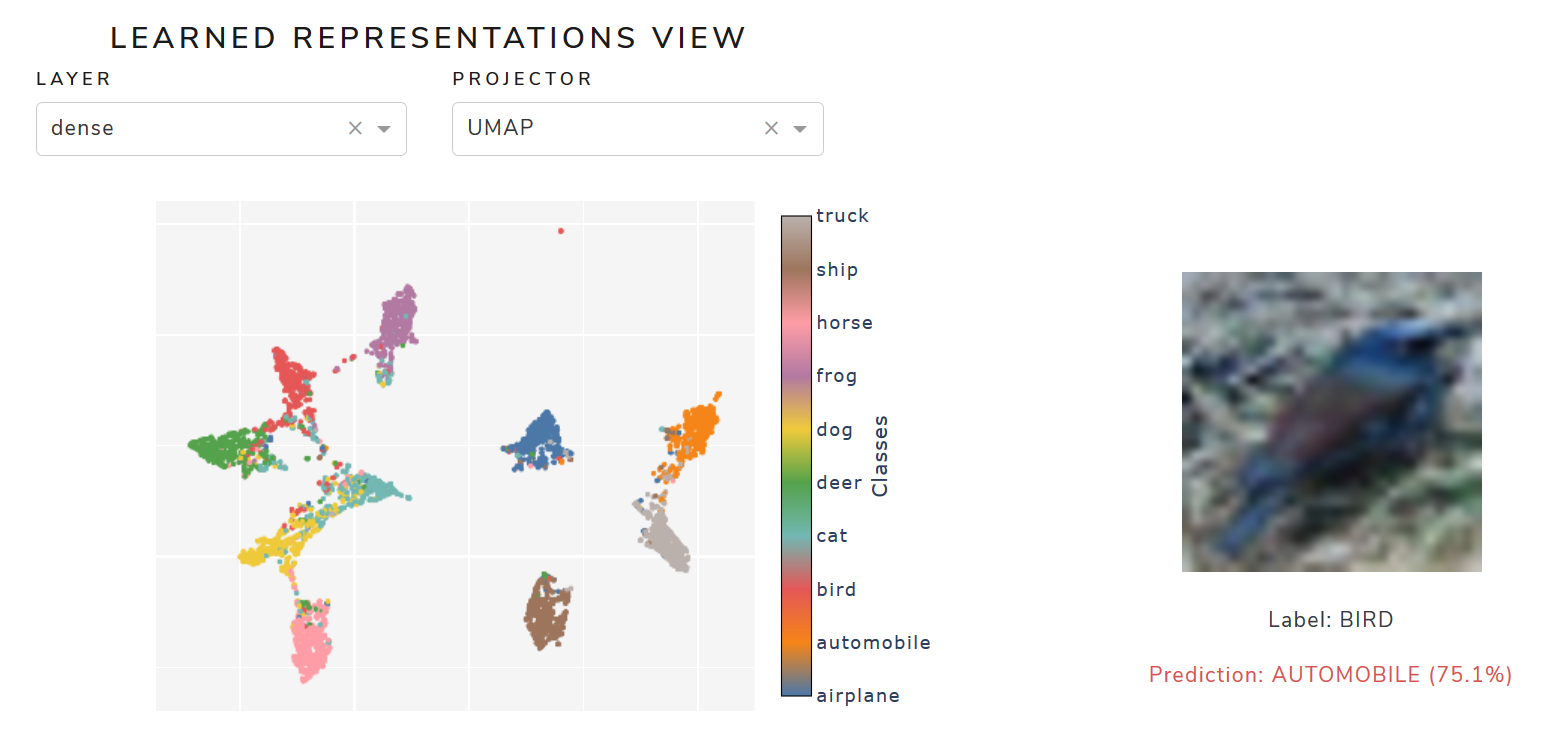
\includegraphics[scale=0.55]{images/embedding_view/HRV_Fig_016_DEV_Layer_Embedding_1.PNG}
	\caption{Deep Embedding Viewer (with Plotly Dash): Learned Representations View with an Incorrect Prediction}
	\label{fig:HRV_016_DEV_Image_Viewer_2}
\end{figure}

\vspace{0.2cm}

Integral to the viewer is the ability to switch between different layers, confirming that moving into increasingly deeper layers leads to increasing specialization within our DCNN:



\vspace{0.4cm}

\begin{figure}[H]
	\begin{minipage}{0.48\textwidth}
		\centering
		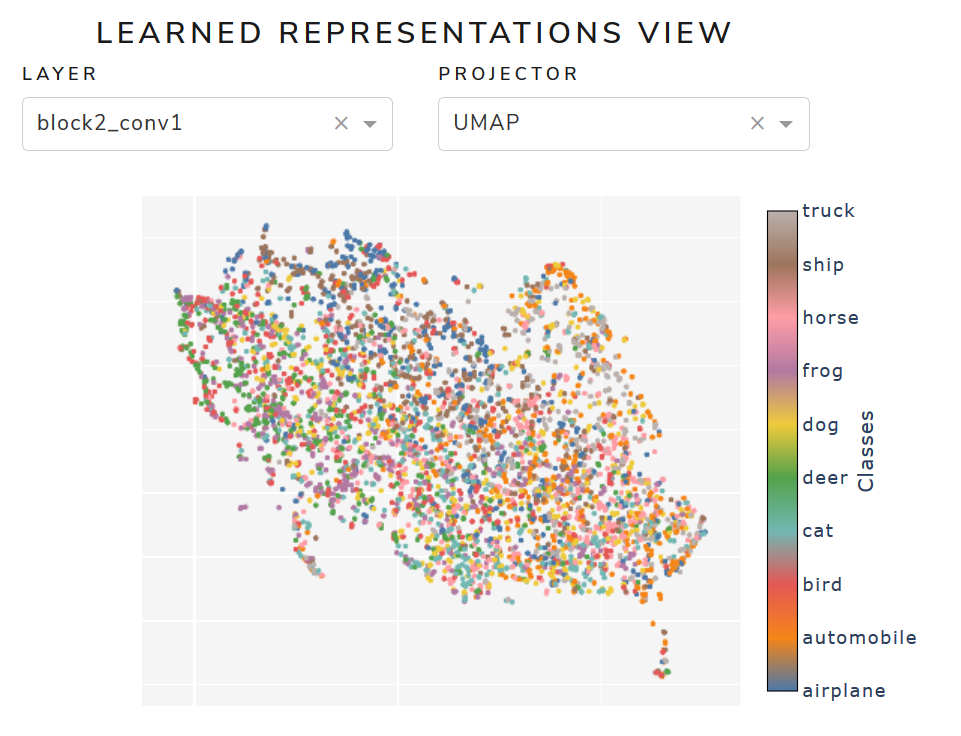
\includegraphics[width=1\linewidth]{images/embedding_view/HRV_Fig_015_DEV_Embedding_4.PNG}
		\caption{UMAP 2D Visualization of VGG-16 block2\_conv1 Convolutional Layer}\label{Fig:HRV_Fig_015_DEV_Embedding_4}
	\end{minipage}\hfill
	\begin{minipage}{0.48\textwidth}
		\centering
		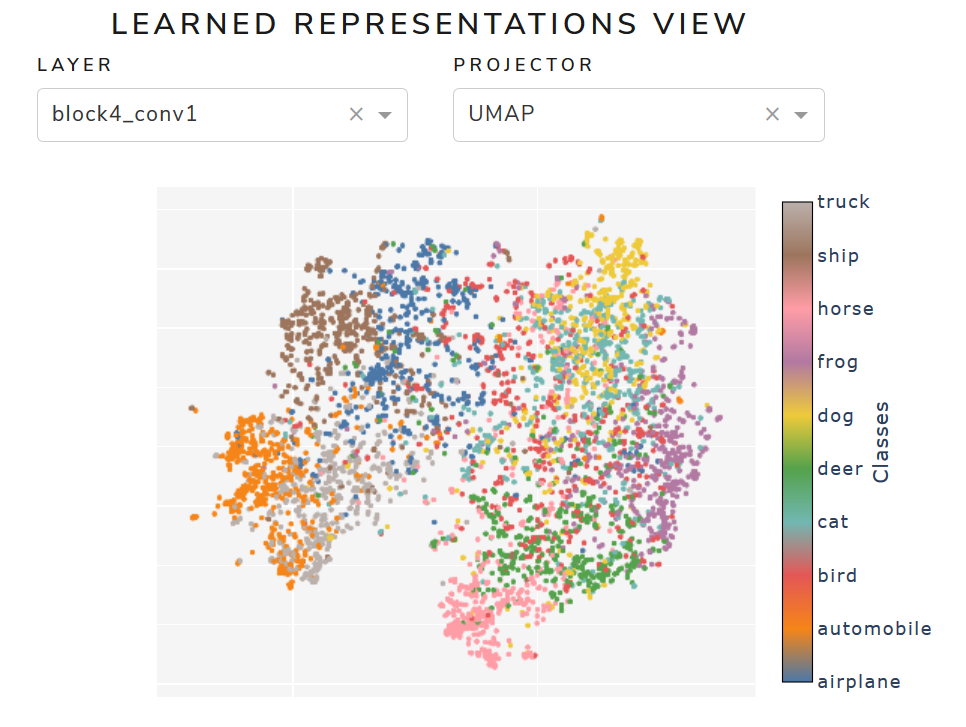
\includegraphics[width=1\linewidth]{images/embedding_view/HRV_Fig_014_DEV_Embedding_3.PNG}
		\caption{UMAP 2D Visualization of VGG-16 block4\_conv1 Convolutional Layer}\label{Fig:HRV_Fig_014_DEV_Embedding_3}
	\end{minipage}
\end{figure}

\vspace{0.2cm}


And different dimensionality reduction methods, e.g. between PCA and UMAP. Although UMAP is the default and preferred approach for our viewer, a more computationally friendly implementation of t-SNE can be used as an alternative:

\vspace{0.2cm}

\begin{figure}[H]
	\begin{minipage}{0.48\textwidth}
		\centering
		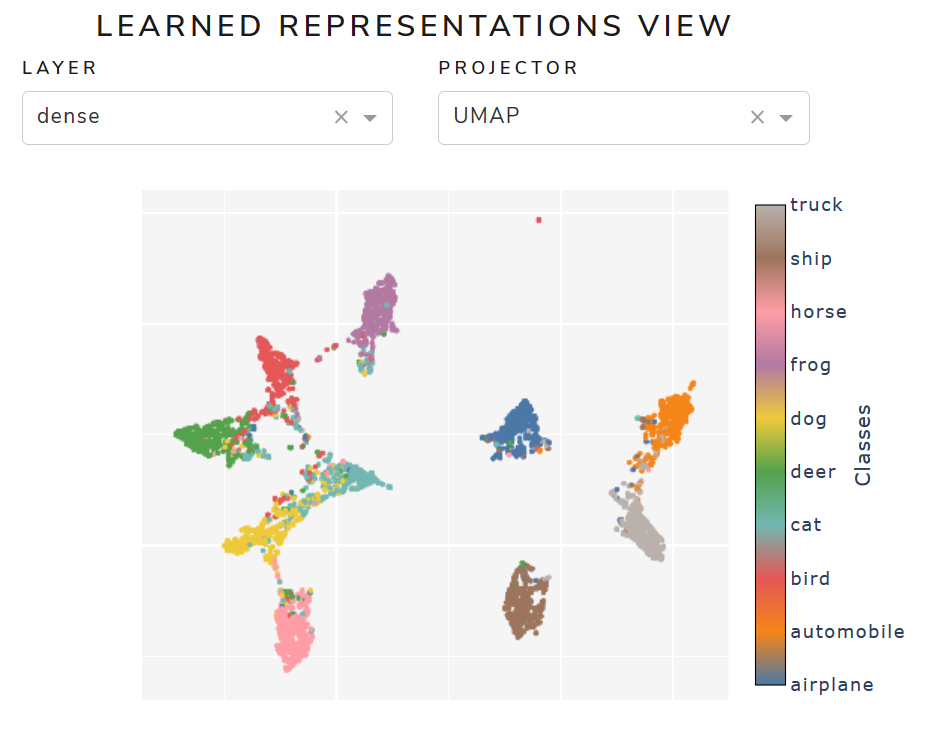
\includegraphics[width=1\linewidth]{images/embedding_view/HRV_Fig_012_DEV_Embedding_1.PNG}
		\caption{UMAP 2D Visualization of VGG-16 Penultimate Dense Layer}\label{Fig:HRV_Fig_012_DEV_Embedding_1}
	\end{minipage}\hfill
	\begin{minipage}{0.48\textwidth}
		\centering
		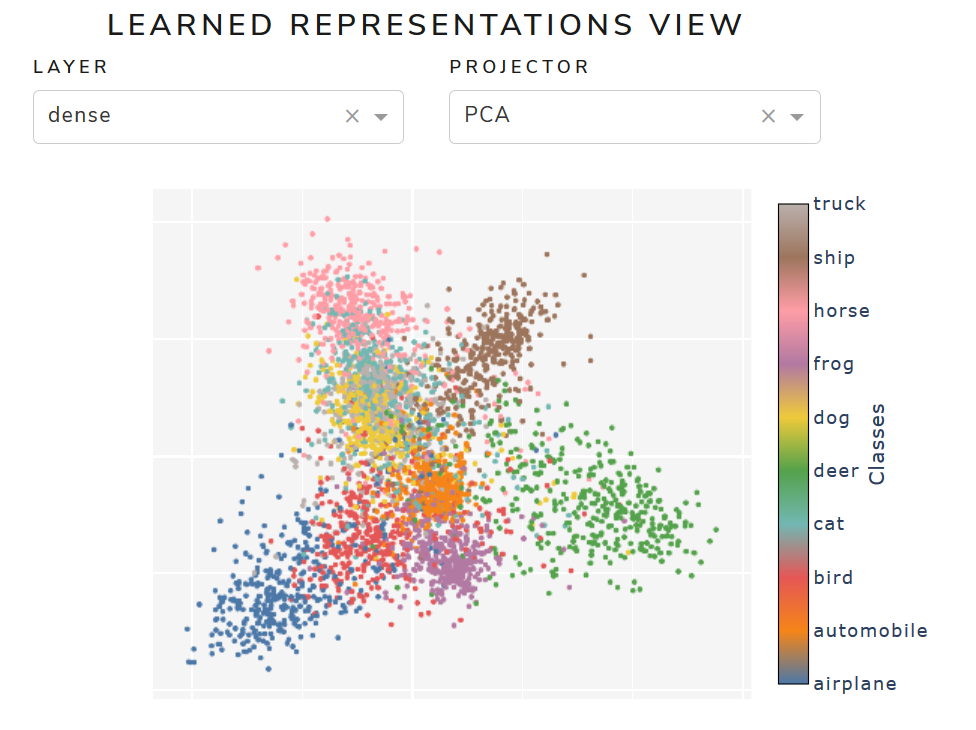
\includegraphics[width=1\linewidth]{images/embedding_view/HRV_Fig_013_DEV_Embedding_2.PNG}
		\caption{PCA 2D Visualization of VGG-16 Penultimate Dense Layer }\label{Fig:HRV_Fig_013_DEV_Embedding_2}
	\end{minipage}
\end{figure}

\vspace{0.2cm}
 
\subsubsection{Deep Embedding Viewer (iii): Neuron Activity Map}

Our application supplements the Learned Representations View with the \textbf{Neuron Activity Map} for visualizing behavioural similarities between neurons and filters (for dense and convolutional layers respectively). Our implementation is a synthesis of three different research papers: (1) the initial blueprint provided by \cite{Rauber2017VisualizingTH}, (2) the use of an alternative distance metric (differing from Pearson correlation) in \cite{Pezzotti2018DeepEyesPV} and (3) the methodology used by \cite{hohman2020summit} for extracting embeddings out of convolutional layers.


For a more detailed description of our implementation, we will start with dense layers. To simplify our analysis of neuron/filter relationships, we start by taking only the absolute values of layer activations. Next, a cosine distance matrix is computed on top of those layer activations. Thus, we obtain the degree of similarity between different neurons (e.g. a layer embedding composed of 10,000 observations described by 200 neurons yields a cosine distance matrix of dimensions $200 \times 200$). This cosine distance matrix is then reduced to 2-dimensional space with the UMAP algorithm (with a specific set of hyperparameters chosen) and plotted on a 2D scatterplot. This entire process is the same for convolutional layers, with the added difference that the methodology from \cite{hohman2020summit} is applied before computing the cosine distance matrix to obtain the necessary convolutional embeddings.


As for our choice to use the cosine distance matrix, it is due to its ability to handle sparse embedding vectors (unlike methods such as the Pearson correlation) and how the output is bounded between 0 and 1. It is also partially due to the fact that the cosine measure is heavily used in the field of NLP for computing the distance between word embeddings.

This panel is directly intertwined with the Learned Representations View, as switching between different layers yields a different view of layer activations and neuron/filter similarities:


\vspace{0.2cm}

\begin{figure}[H]
	\begin{minipage}{0.48\textwidth}
		\centering
		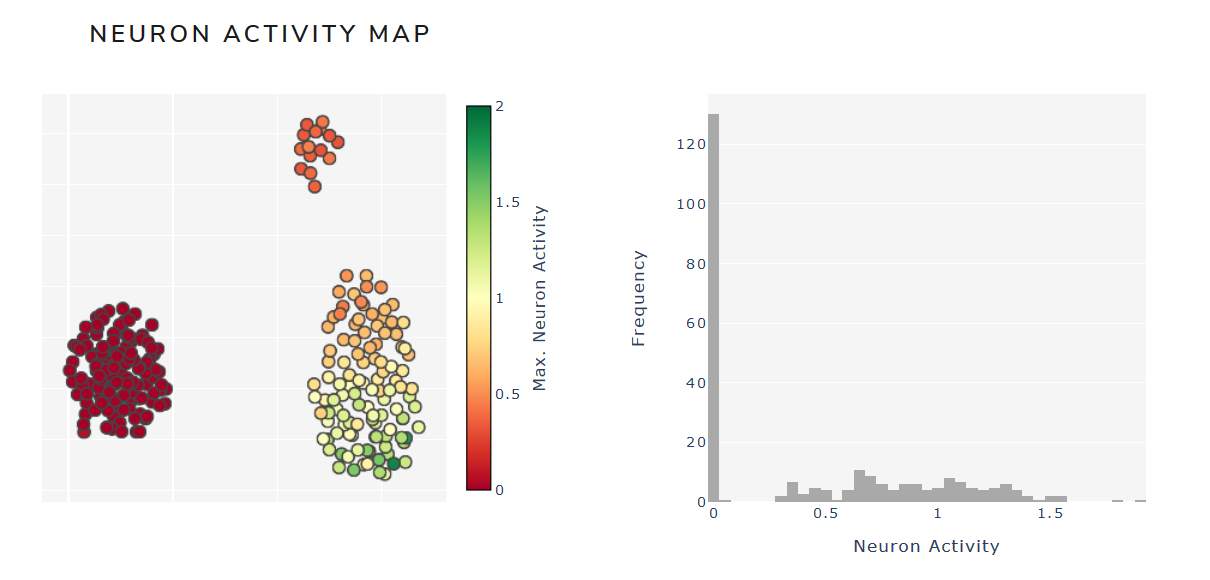
\includegraphics[width=1\linewidth]{images/embedding_view/HRV_Fig_017_DEV_Neuron_Embedding.PNG}
		\caption{UMAP 2D Visualization of VGG-16 Penultimate Dense Layer Neurons}\label{Fig:HRV_Fig_017_DEV_Neuron_Embedding}
	\end{minipage}\hfill
	\begin{minipage}{0.48\textwidth}
		\centering
		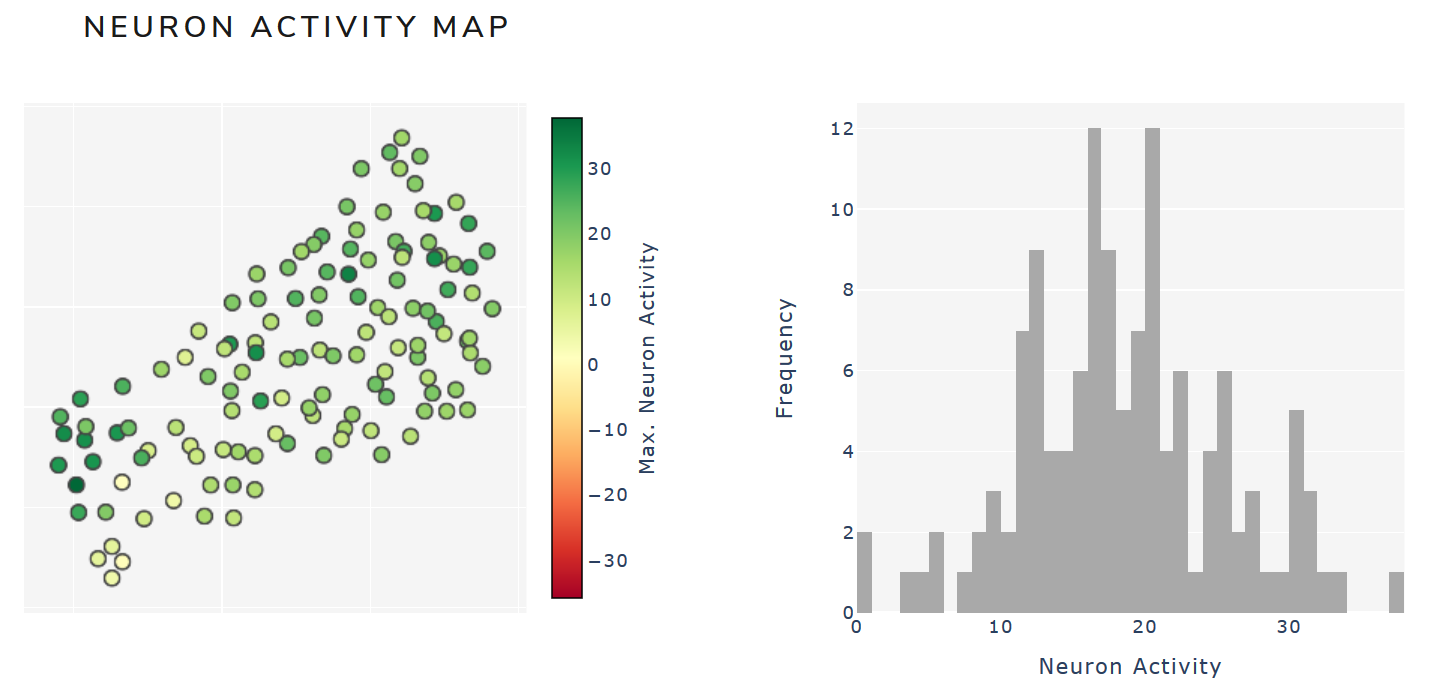
\includegraphics[width=1\linewidth]{images/embedding_view/HRV_Fig_018_DEV_Neuron_Embedding_2.PNG}
		\caption{UMAP 2D Visualization of VGG-16 block4\_conv1 Filters}\label{Fig:HRV_Fig_018_DEV_Neuron_Embedding_2}
	\end{minipage}
\end{figure}


\vspace{0.2cm}

Unlike the Learned Representations View, UMAP is the only provided option for visualizing neuron/filter similarities.

\subsubsection{Deep Embedding Viewer (iv): Model Performance Analysis}

Our initial viewer lacked basic information on the DCNN's actual performance. Thus, we supplement the previous visualizations with simple but effective performance metrics - \textbf{Normalized Confusion Matrix} and \textbf{Class Prediction Accuracy} - that will help the user understand the results obtained in the Learned Representations View and Neuron Activity Map. Visual clutter in the Learned Representations View when visualizing the penultimate layers before softmax classification is likely to be indicative of label confusion (e.g. dogs confused as cats in the case of CIFAR-10), which can be confirmed with the confusion matrix.




\vspace{0.2cm}

\begin{figure}[H]
	\centering
	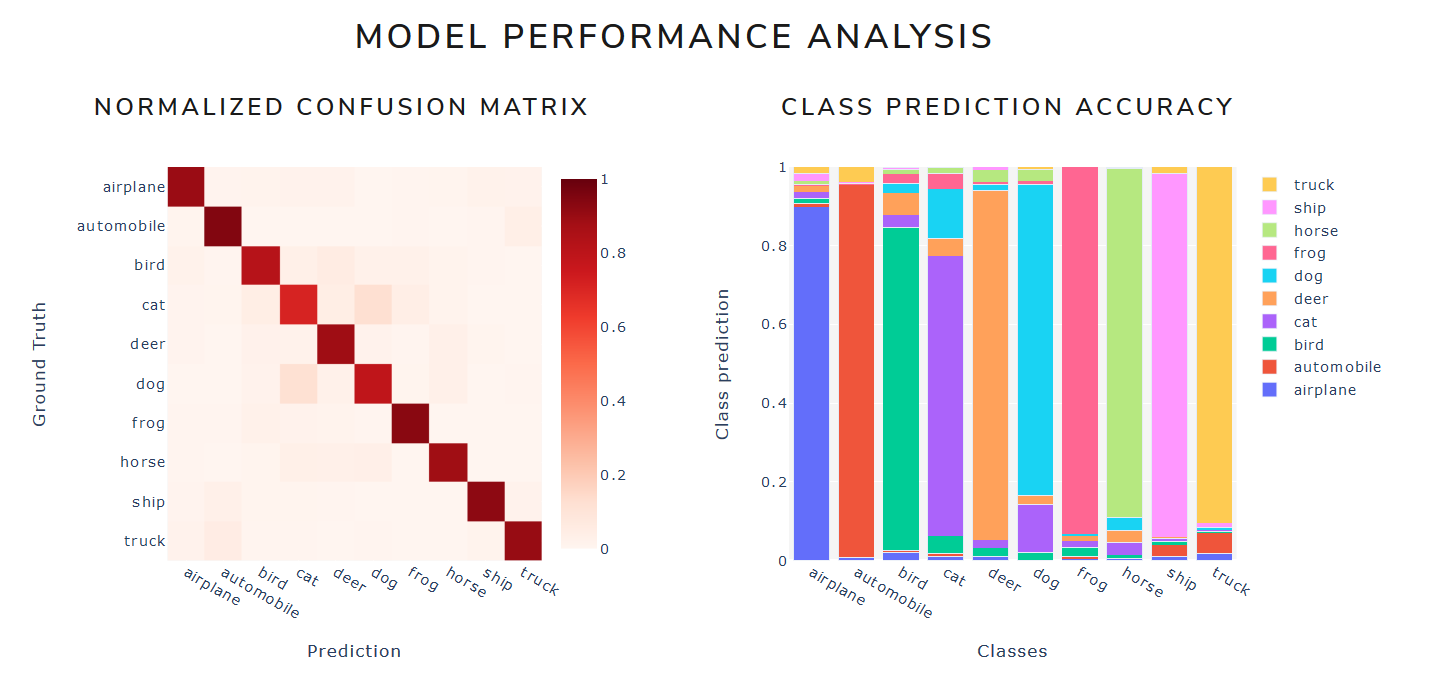
\includegraphics[scale=0.55]{images/embedding_view/HRV_Fig_011_DEV_Metrics.PNG}
	\caption{Deep Embedding Viewer (with Plotly Dash): Model Performance Analysis}
	\label{fig:HRV_Fig_011_DEV_Metrics}
\end{figure}

\vspace{0.2cm}

Complementing embedding visualization with performance metrics is also further recommended by 
\cite{Rauber2017VisualizingTH} for improving the reliability and the relevance of embedding visualization.


\subsubsection{Deep Embedding Viewer (v): Adversarial Robustness Simulation}

Although elaborated in greater detail in a previous section, \textbf{Adversarial Robustness Simulation} is provided as an additional panel (at the end of the viewer) for stress testing convolutional neural networks against FGSM-generated adversarial attacks.

